\chapter{励磁}
\section{引言}
本章我们使用Bean于1962年提出的唯象磁化理论来讨论第II类超导体的磁化问题。如第一章指出的,对多数超导磁体应用所关注的磁场范围($>\sim 0.5T$),第II类超导体
处于混合态,即在超导态的“海”中还存在正常态的“岛”。当第II类超导体处于时变磁场或时变传输电流中时,这些岛中将产生耗散,体现为磁通跳跃(一种暂态现象)或交流损耗。
所谓的Bean临界态模型,以闭式表达式阐明了消除磁通跳跃和最小化交流损耗的必要条件。

如今,已经有了可以完全消除磁通跳跃的生产LTS线/缆的成熟方法。我们在本章将学习到,磁通跳跃在HTS中并不像在LTS中是那么重要。如果仅在消除磁通跳跃方面磁化是重要的,
那在HTS应用中可将其视为次要考虑问题。然而,由于磁化在LTS和HTS的交流损耗中也起到重要作用,所以我们用一章来研究它。交流损耗将在第七章有更详细的讨论。

\section{第II类超导体的Bean理论}
\subsection{无传输电流}
和很多成功的理论一样,Bean模型通过一些假设,可用简单的数学推导出闭式表达式,与实验结果取得了很好的一致性。在Bean模型中,超导体有最简单的几何结构——
$x$方向宽度为$2a$,$y$和$z$向无限长。磁场($H, B, M$)指向y向,而电流($I, J$)在z向流动。在Bean模型中,$J=J_c$(临界电流密度),并假定其不依赖于磁场和温度。

于是,磁场本构关系可以简化为下式:
\begin{equation}
  M=\frac{B}{\mu_0} -H
\end{equation}

根据Bean模型,磁感应强度B在硬超导体内的次表面内不为0,而是等于超导体的体平均$\mu_0 H_s$,$H_s$是超导体内的磁场。

%%图5.1
\begin{figure}[htbp]
  \centering
 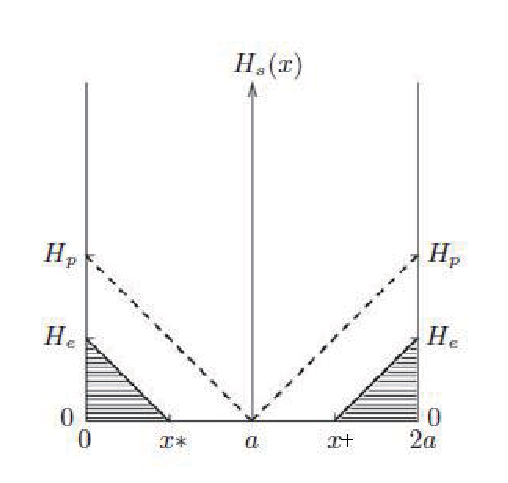
\includegraphics[scale=0.8]{chpt5/figs/fig5.1.eps}
  \caption{置于外磁场中的第II类超导体板}\label{fig:slabinfield}
\end{figure}
图\ref{fig:slabinfield}展示了第无限高($y$向)、无限深($z$向)、$2a$宽($x$向)第II类超导体板的。板此前未处于磁场中,外磁场$H_e$平行于板施加,将在板内产生$H_s(x)$。
根据安培定律$\nabla \times H = J=J_c$,我们可以得到超导体内的磁场$H_s(x)$:
%\begin{equation}
%  H_s(x)=
%  \begin{cases}
%           0, & \mbox{x*\le x \le x+ }  \\
%           H_e - J_c x, & \mbox{0\le x \le x* } \\
%           H_e + J_c (x-2a), & \mbox{x+ \le x \le 2a}
%   \end{cases}
%\end{equation}
注意到,$H_s(x)$的斜率等于$J_c$,当$J_c$大于0时(z向,朝向纸面外)大于0,$J_c$小于0时小于0。$x*$和$2a-x^+$给出磁场的穿透程度,表示为
\begin{equation}
  x*=\frac{H_e}{J_c}
\end{equation}

在$H_e=H_p\equiv J_c a$时,$x^*=x^+=a$,整个板处于临界态。$H_p$是所谓的穿透磁场,定义为
\begin{equation}
  H_p\equiv J_c a
\end{equation}

板内的平均磁感应强度由下式给出:
\begin{equation}
\begin{split}
\~{B}_s&=\frac{\mu_0}{2a}\int_{0}^{2a} H_s(x)dx \\
&=\frac{\mu_0}{2a}\times <\mbox{图5.1中的阴影面积}> \\
&=2\times \frac{\mu_0}{2a}\times \frac{H_e x^*}{2}=\frac{\mu_0 H_e^2}{2aJ_c}\\
&=\frac{\mu_0 H_e^2}{2H_p}
\end{split}
\end{equation}

根据定义$M=~{B}_s / \mu_0-H_e$,可得
\begin{equation}
  -M=H_e-\frac{H_e^2}{2H_p},(0\le H_e \le H_p)
\end{equation}

超导体是抗磁性的,-M是它的磁化强度。

随着外磁场的进一步增加,磁场将最终穿透整个板($H_e\ge H_p$),根据$~{B}_s=H_e-H_p/2$,有
\begin{equation}
  -M=\frac{1}{2}H_p=\frac{1}{2}J_c a, (H_e\ge H_p)
\end{equation}

图中的虚线磁化线对应$H_e=H_p$情况。
%5.2
\begin{figure}[htbp]
  \centering
 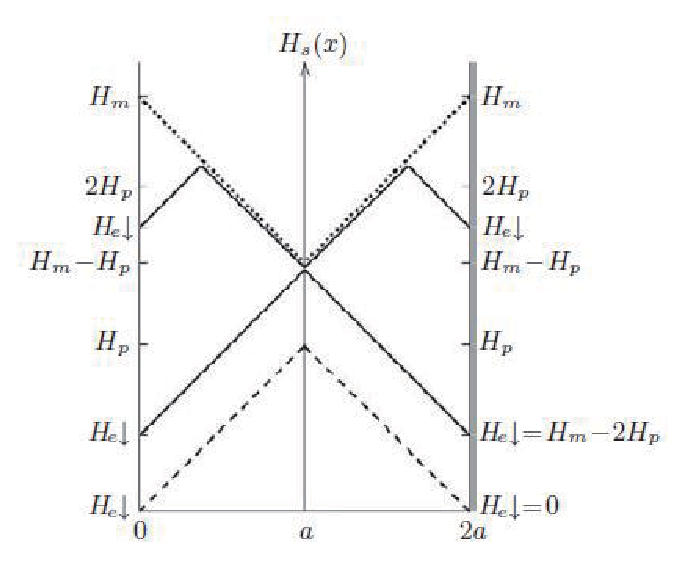
\includegraphics[scale=0.8]{chpt5/figs/fig5.2.eps}
  \caption{退场过程中的$H_s(x)$:$H_e\downarrow=H_m\rightarrow 0$}\label{fig:hreturn}
\end{figure}

图\ref{fig:hreturn}中的点线表示的是$H_s(x)$在$H_e=H_m>2H_p$时的情况。其中,$H_m$是外施磁场序列的最大值。

当$H_e$从$H_m$减至0的过程中,$H_s(x)$如图\ref{fig:hreturn}中的实线所示。当$H_e=H_m-2H_p$时,$-M$成为$-H_p /2$。
可以看到,外场从$H_m$到$H_e\downarrow=0$的退场过程中,$-M(H_e)$由下式给出
\begin{eqnarray}
% \nonumber % Remove numbering (before each equation)
  -M(H_e) =&\frac{1}{2}H_p-(H_m-H_e)+\frac{(H_m-H_e)^2}{4H_p}\\ \nonumber
                 & ,(H_e\downarrow=H_m\rightarrow H_m-2H_p) \\ \nonumber
  -M(H_e) =&-\frac{1}{2}H_p,\quad (H_e\downarrow=H_m-2H_p\rightarrow 0)
\end{eqnarray}

当外场施于“纯”板时,$-M$是$H_e$的二次函数。而在$H_e$退回0时,$-M(H_e)=-H_p /2$。“剩余”磁化如图\ref{fig:hreturn}中的虚划线所示。可知当置于外场中,
第II类超导体将会被磁化。剩余磁场不能通过外施磁场的方法去除。一种去除它的方法是加热超导体至临界温度$T_c$以上。
%5.3
\begin{figure}[htbp]
  \centering
 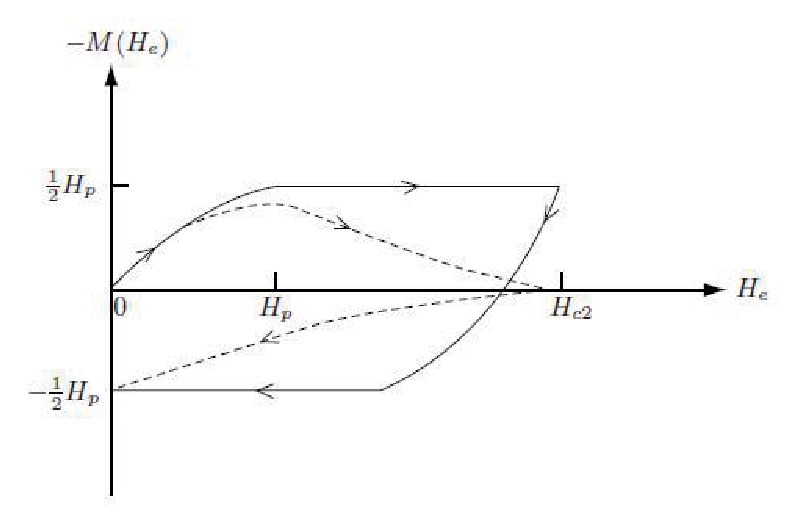
\includegraphics[scale=0.8]{chpt5/figs/fig5.3.eps}
  \caption{某硬超导体在外磁场($0\rightarrow H_{c2}\rightarrow 0$)下的磁化和磁场的关系。
  其中,实线表示$J_c=const$;虚线定性表示了电流随磁场下降的事实。}\label{fig:magvsh}
\end{figure}
图\ref{fig:magvsh}给出了完整的磁场从0增至$H_m=H_{c2}$又退回0的完整图像。其中,$H_{c2}$是超导体的上临界场。实线是基于由Bean的关于$J_c$不依赖磁场的假设
而导出的5.5-5.7式确定的。虚划线是对更接近实际情况的定性修正,反映了$J_c$随磁场衰减的事实,在$H_{c2}$时为0。注意到,磁化是有回滞的,在
$H_p<H_e<H_m-2H_p,\quad \Delta M=-M(H_e\uparrow)+M(H_e\downarrow)$范围内,磁场的幅值为$H_p=J_c a$。
于是,有时通过获得$J_e(H_e)$数据来做磁化的测量。
%5.4
\begin{figure}[htbp]
  \centering
 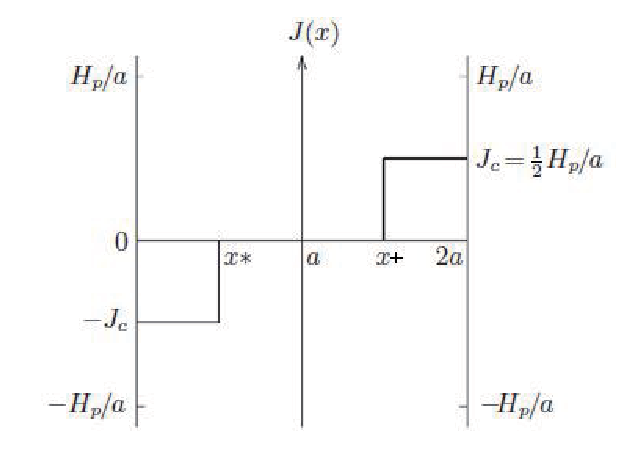
\includegraphics[scale=0.8]{chpt5/figs/fig5.4.eps}
  \caption{在图5.1给出的磁场$H_s(x)$下的$J(x)$}\label{fig:jtoh}
\end{figure}
图\ref{fig:jtoh}给出了在施加图\ref{fig:slabinfield}分布磁场下的板内电流分布。注意到$J_c=H_p /2a$。$y$向的单位长度净电流沿板的$z$向流动,由下式给出
\begin{equation}
  I=\int_{0}^{2a} J(x)dx=0
\end{equation}

\subsection{传输电流对励磁的效应}
当有传输电流$I_t$($y$向单位长度)在板中沿$+z$方向(流出纸面)时,我们看到在$x=2a$处磁场有一个$I_t/2$的增长,在$x=0$处有一个$I_t/2$的减少。

因为板内屏蔽电流是从每一个表面逐渐进入内部的,板内的场分布$H_s(x)$如图\ref{fig:hwithi}所示。图中的$x^*$和$x^+$由下式给出:
\begin{eqnarray}
% \nonumber % Remove numbering (before each equation)
  -\frac{1}{2}I_t + J_c x^* = 0 \\ \nonumber
  J_c(x^*-2a)+\frac{1}{2}I_t = 0 \\ \nonumber
  x^*=\frac{I_t}{2J_c}\quad \& \quad x^+ = 2a-\frac{I_t}{2J_c}
\end{eqnarray}

%%%%图5.5
\begin{figure}[htbp]
  \centering
 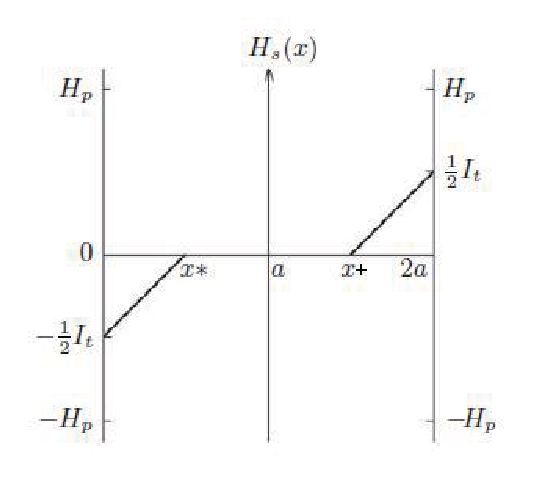
\includegraphics[scale=0.8]{chpt5/figs/fig5.5.eps}
  \caption{板内存在传输电流$I_t$时的磁场$H_s(x)$}\label{fig:hwithi}
\end{figure}

图5.6给出了板内的电流分布$J(x)$。沿着板宽度方向积分,我们可以得到板内的净电流就是$I_t$:
\begin{equation}
  I=\int_{0}^{2a}J(x)dx=J_c x^*+J_c(2a-x^+)=1/2 I_t +1/2 I_t=I_t
\end{equation}

\begin{figure}[htbp]
  \centering
 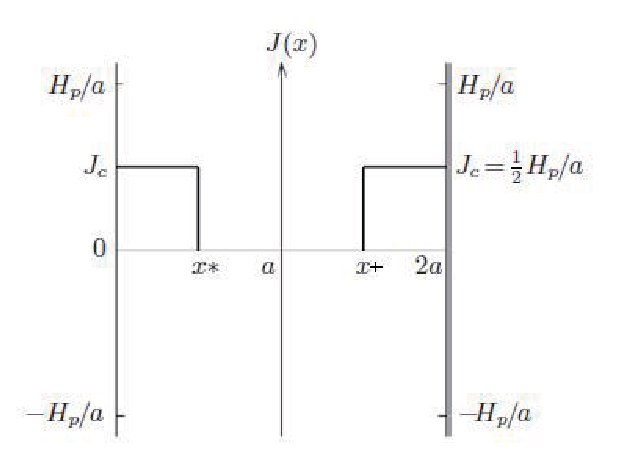
\includegraphics[bb=0 0 800 600]{chpt5/figs/fig5.6.eps}
  \caption{在图5.5给出的磁场$H_s(x)$下的$J(x)$}\label{fig:jtoh5.5}
\end{figure}

也即,板内的净电流就是外施电流。注意到,若外磁场$H_e\vec{i_y}$在$I_t$通入后施加,基本不会改变电流的分布(图5.5和5.6);但若外磁场
先于电流施加,则会出现不同的$H_s(x)$和$J(x)$。

\section{测量技术}
这里我们描述最经常使用的测量磁化的技术。图5.7指示了本项技术的关键组件:1)初级查找线圈;2)次级查找线圈;3)平衡分圧计。
图中未画出但也同等重要的是积分器,它将桥路输出电压$V_bg$转换为直接正比于$M(H_e)$的电压信号。测试样品置于初级查找线圈内,。
当初级查找线圈和次级查找线圈置于在两个线圈所占的空间内基本均匀的时变外磁场$H_e(t)$中,各查找线圈的端子上将出现感应
电压$V_{pc}(t)$和$V_{sc}(t)$:
\begin{eqnarray}
% \nonumber % Remove numbering (before each equation)
  V_{pt}(t) &=& \mu_0 N_{pc} A_{pc}\left[ \frac{dM}{dt}+(\frac{d\~{H}_e}{dt})_{pc}\right] \\ \nonumber
  V_{sc}(t) &=& \mu_0 N_{sc} A_{sc}\left( \frac{d\~{H}_e}{dt}\right)_{sc}
\end{eqnarray}

下标pc和sc分别表示初级线圈(primary coil)和次级线圈(second coil)。N是各线圈的匝数。A是耦合$H_e(t)$的每一匝线圈的有限面积。
$\~{H}_e$是磁场在各线圈内的空间平均值。

桥输出电压$V_bg$由下式给出:
\begin{equation}
  V_{bg}(t)=(k-1)V_{pt}(t)+kV_{sc}(t)
\end{equation}

其中,k是一个介于0-1的常数,表示分压计在初级线圈侧的分压系数(图5.7)。联立上两式,可得
\begin{equation}
  V_{bg}(t)=(k-1)\mu_0 N_{pc}A_{pc}\frac{dM}{dt}+(k-1)\mu_0 N_{pc}A_{pc}(\frac{d\~{H}_e}{dt})_{pc}+k\mu_0 N_{sc}A_{sc}(\frac{d\~{H}_e}{dt})_{sc}
\end{equation}

%%图5.7
\begin{figure}[htbp]
  \centering
 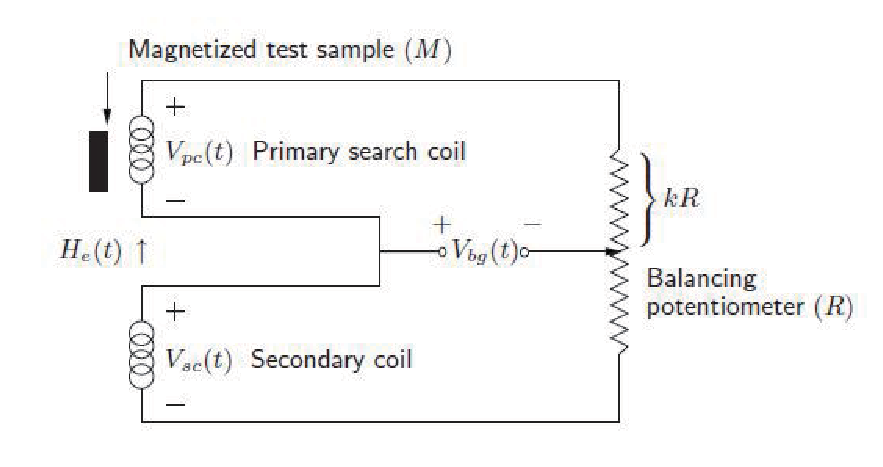
\includegraphics[scale=0.8]{chpt5/figs/fig5.7.eps}
  \caption{磁化测量原理图}\label{fig:magmeasure}
\end{figure}

通过调节分压系数k可以满足以下条件,令$V_{bg}(t)$正比于$dM/dt$:
\begin{eqnarray}
% \nonumber % Remove numbering (before each equation)
  &(k-1)\mu_0 N_{pc}A_{pc}(\frac{d\~{H}_e}{dt})_{pc}+k\mu_0 N_{sc}A_{sc}(\frac{d\~{H}_e}{dt})_{sc}=0 \\ \nonumber
  &V_{bg}(t)=(k-1)\mu_0 N_{pc}A_{pc}\frac{dM}{dt}
\end{eqnarray}

尽管实际上上式第一式所给的归零条件在很大范围内不是总能满足,但是第二式对多数情况都是很好的近似。
一般,$k$接近0.5。$V_bg{t}$馈入一个积分器,其输出正比于$M$。特别的,如果样品是“纯”的($M=0$),磁场
$H_e(t)$从0($t=0$)增($\uparrow$)至$H_e$($t=t_1$)时,我们有
\begin{equation}
  V_{mz}(H_e\uparrow)=\frac{1}{\tau_{it}}\int_{0}^{t_1}V_bg(t)dt=\frac{(k-1)\mu_0 N_{pc}A_{pc}}{\tau_{it}}M(H_e)
\end{equation}

式中,$\tau_{it}$是有效积分常数。如果$H_e>H_p$,此时有$M(H_e)=-H_p / 2=-J_c a / 2$,则上式简化为
\begin{equation}
    V_{mz}(H_e\uparrow>H_p)=-f_m \frac{(k-1)\mu_0 N_{pc}A_{pc}}{\tau_{it}}(\frac{J_c a}{2})
\end{equation}

因数$f_m$是磁性材料体积与样品总体积之比。之所以需要这个因数是因为待磁化测试的样品一般不全是由磁性材料组成。
比如多丝(层)导体,样品除了超导丝(层)外,还存在基底金属和其他非磁性材料。如果外场按$0\rightarrow H_m>H_p\rightarrow H_e\downarrow <H_m-2H_p$顺序,
我们有
\begin{equation}
    V_{mz}(H_e\downarrow<H_m-2H_p)=-f_m \frac{(k-1)\mu_0 N_{pc}A_{pc}}{\tau_{it}}(\frac{J_c a}{2})
\end{equation}

于是,$\Delta V_{mz}=V_{mz}(H_e>H_p)-V_{mz}(H_e\downarrow<H_m-2H_p)$正比于在$H_e$处磁化曲线的“宽度”:
\begin{equation}
    \Delta V_{mz}=-f_m \frac{(k-1)\mu_0 N_{pc}A_{pc}}{\tau_{it}} J_c a
\end{equation}

上式我们看出,$\Delta V_{mz}$是直接正比于$J_c$和$a$的。
%%图5.8
\begin{figure}[htbp]
  \centering
 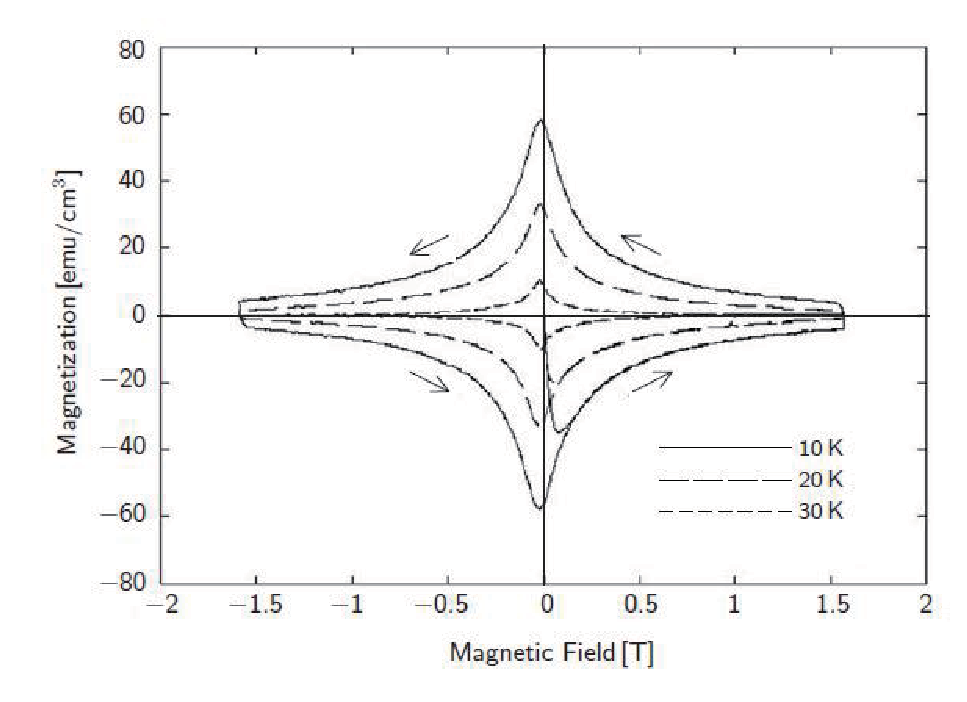
\includegraphics[scale=0.7]{chpt5/figs/fig5.8.eps}
  \caption{$MgB_2$在$10K,20K,30K$三种温度下的磁化和磁场关系}\label{fig:magvfield}
\end{figure}
图5.8给出的是$MgB_2$在10K,20K,30K时,磁场按$0\rightarrow 1.7T\rightarrow 0 \rightarrow -1.7T\rightarrow 0$完整施加时的磁化与磁场的关系。注意到,
和图5.3不同,本图中还有$+M(H_e)$。因为凸显在$x$轴上(磁场)并不偏斜,我们可以认为本测试中初次、二次线圈已得到很好的平衡。

磁化的回滞表明,$MgB_2$是第II类超导体,它的抗磁性在每一个图线的第一部分(磁场从0增至1.7T时)明显可见。

从Bean模型可知,$H_p=J_c a$,即磁化直接正比于$J_c$。然而,实际上$J_c$不仅是磁场还是温度的减函数。图5.8中明显可见对$J_c$和$T$的依赖。
图中的$M$的单位是$emu/cm^3$,不是SI单位。

\section{专题}
\subsection{讨论5.1:传导电流磁化}
正如本书最初所述,在传输电流存在条件下的励磁依赖于外场和传输电流施加的顺序。
这里我们考虑三种情况:A) 先加磁场后加传输电流; B) 先通电流后加磁场;C) 磁场和电流交替改变。

\textbf{A.  先加磁场后加传输电流}

\begin{equation}% page321 第1个
H_{s2_{1}}(x)=2H_{p}+J_{c}x=2J_{c}a+J_{c}x\qquad(0\leq x\leq x*)
\end{equation}
\begin{equation}% page321 第2个
H_{s2_{2}}(x)=2.5H_{p}-J_{c}x=2.5J_{c}a-J_{c}x\quad(x*\leq x\leq x+)
\end{equation}
\begin{equation}% page321 第3个
H_{s2_{3}}(s)=H_{p}+J_{c}x=J_{c}a+J_{C}x\qquad(x+\leq x\leq 2a)
\end{equation}
\begin{equation}% page322 第1个
H_{s2_{1}}(X)=(H_{e}-\frac{1}{2}I_{t})+J_{c}x\qquad(0\leq x\leq x*)
\end{equation}
\begin{equation}% page322 第2个
H_{s2_{2}}(x)=H_{e}-J_{c}x\qquad(x*\leq x\leq x+)
\end{equation}
\begin{equation}% page322 第3个
H_{s2_{s}}(x)=(H_{e}+\frac{1}{2}I_{t})+J_{c}(x-2a)\qquad(x+\leq x\leq2a)
\end{equation}
\begin{equation}% page322 第4个
H_{{s}2_{1}}(x*)=H_{s2_{2}}(x*)
\end{equation}
\begin{equation}% page322 第5个
H_{e}-H_{p}i+J_{c}x*=H_{e}J_{c}x*\Rightarrow x*=\frac{H_{p}}{2J_{c}}i=\frac{1}{2}ai
\end{equation}
\begin{equation}% page322 第6个
H_{s2_{2}}(x*)=H_{e}-\frac{1}{2}aJ_{c}i=H_{e}-\frac{1}{2}H_{p}i
\end{equation}
\begin{equation}% page322 第7个
H_{s2_{2}}(x+)=H_{s2_{3}}(x+)
\end{equation}
\begin{equation}% page322 第8个
H_{e}-J_{c}x+=H_{e}+H_{p}i+J_{c}(x^{+}-2a)\Rightarrow x^{+}=a(1-\frac{1}{2}i)
\end{equation}
\begin{equation}% page322 第9个
H_{s2_{2}(x+)}=H_{e}-H_{p}+\frac{1}{2}H_{p}i
\end{equation}
\begin{equation}% page323 第1个
A_{1}=\frac{1}{2}x*[H_{s1}(0)+H_{s2}(x*)]=\frac{1}{4}ai[(H_{e}-H_{p}i)+(H_{e}-\frac{1}{2}H_{p}i)]\\
=\frac{1}{4}ai(2H_{e}-\frac{3}{2}H_{p}i)  
=a(\frac{1}{2}H_{e}i-\frac{3}{8}H_{P}i^{2})
\end{equation}
\begin{equation}% page323 第2个
A_{2}=\frac{1}{2}(x^{+}-x*)[H_{s2}(x*)+H_{s2}(x^{+})]\\
=\frac{1}{2}(a-ai)(H_{e}-\frac{1}{2}H_{p}i+H_{e}-H_{p}+\frac{1}{2}H_{p}i)\\
=\frac{1}{2}a(-i)(2H_{e}-H_{p})\\
=a(H_{e}-H_{e}i-\frac{1}{2}H_{p}+\frac{1}{2}H_{p}i)
\end{equation}
\begin{equation}% page323 第3个
A_{3}=\frac{1}{2}(2a-x+)[H_{s2}(x+)+H_{s3}(2a)]\\
=\frac{1}{2}(a+\frac{1}{2}ai)(H_{e}-H_{p}+\frac{1}{2}H_{p}i+H_{e}+H_{P}i)\\
=a(1+\frac{1}{2}i)(H_{e}-\frac{1}{2}H_{p}+\frac{3}{4}H_{p}i)\\
=a(H_{e}+\frac{1}{2}H_{e}i-\frac{1}{2}H_{p}-\frac{1}{4}H_{p}i+\frac{3}{4}H_{p}i+\frac{3}{8}H_{p}i^{2})
\end{equation}
\begin{equation}% page323 第4个
Shaded\quad area=A_{1}+A_{2}+A_{3}\\
=a(\frac{1}{2}H_{e}i-\frac{3}{8}H_{p}i^{2}+H_{e}-H_{e}i-\frac{1}{2}H_{p}+\frac{1}{2}H_{p}i\\
+H_{e}+\frac{1}{2}H_{e}i-\frac{1}{2}H_{p}-\frac{1}{4}H_{P}i+\frac{3}{4}H_{P}i+\frac{3}{8}H_{p}i^{2})\\
=a(2H_{e}-H_{p}+H_{p}i)
\end{equation}
\begin{equation}% page323 第4个
-M(i)=H_{e}-\frac{1}{2a}\times(Shaded\quad area)\\
=H_{e}-H_{e}+\frac{1}{2}H_{p}-\frac{1}{2}H_{p}i\\
=\frac{1}{2}H_{p}(1-i)\qquad(5.17a)\\
=-M(0)f_{1}(i)\qquad(5.17b)
\end{equation}

C) 磁场和电流交替改变。

\textbf{B. 先通电流后加磁场}

\begin{equation}% page324 第1个
I_{t}=\int_{0}^{2a}J(x)dx=J_{c}(0.5)+J_{c}(2a-1.5a)=J_{c}a
\end{equation}
\begin{equation}% page324 第2个
I_{t}=\int_{0}^{2a}J(x)dx=-J_{c}(0.5a)+J_{c}(2a-0.5a)=J_{c}a
\end{equation}
\begin{equation}% page324 第3个
H_{s1}(x)=(H_{e}-H_{p}i)-J_{c}x\qquad(0\leq \leq x*)
\end{equation}
\begin{equation}% page324 第4个
H_{s2}(x)=(H_{e}+H_{p}i)+J_{c}(x-2a)\quad(x*\leq x leq  2a)
\end{equation}
\begin{equation}% page324 第5个
x*=a-ai=a(1-i)
\end{equation}
\begin{equation}% page325 第1个
H_{s1}(x*)=H_{e}-H_{p}i-J_{c}a(1-i)=J_{e}-H_{p}
\end{equation}
\begin{equation}% page325 第2个
A_{1}=\frac{1}{2}a(1-i)(H_{e}-H_{p}i+H_{e}-H_{p}\\
=a(1-i)(H_{e}\frac{1}{2}H_{p}-\frac{1}{2}H_{p}i)\\
=a(H_{e}-H_{e}i\frac{1}{2}H_{p}+\frac{1}{2}H_{p}i^{2})
\end{equation}
\begin{equation}% page325 第3个
A_{2}=\frac{1}{2}(2a-a+ai)(H_{e}+H_{p}i+H_{e}-H_{P})\\
=a(1+i)(H_E-\frac{1}{2}H_{p}+\frac{1}{2}H_{p}i)\\
=a(H_{e}+H_{e}-\frac{1}{2}H_{p}+\frac{1}{2}H_{p}i^{2})
\end{equation}
\begin{equation}% page325 第4个
Shaded\quad area=A_{1}+A_{2}\\
=a(2H_{e}-H_{p}+H_{p}i^{2})
\end{equation}
\begin{equation}% page325 第5个
-M(i)=H_{e}-\frac{1}{2}(2H_{e}-H_{p}+H_{P}i^{2}\\
=\frac{1}{2}H_{p}(1-i^{2})\qquad(5.18a)\\
=-M(0)f_{2}(i)\qquad(5.18b)
\end{equation}


\textbf{C. 磁场和电流交替改变}

\begin{equation}% page326 第1个
H_{s2}(x)=H_{e}+H_{p}i-J_{c}x\qquad(x*\leq x\leq a)\\
\end{equation}

\begin{equation}% page326 第2个
H_{s3}(x)=H_{e}+H_{p}i+J_{c}(x-2a)\quad(a\leq x\leq a^{+})\\
\end{equation}

\begin{equation}% page326 第3个
H_{s2}(x*)=H_{e}\Rightarrow H_{e}+H_{p}i-J_{c}x*\\
\end{equation}

\begin{equation}% page326 第3个
x*=\frac{H_{p}i}{J_{c}}=ai\\
\end{equation}

\begin{equation}% page326 第4个
H_{s3}(x+)=H_{e}\Rightarrow H_{e}+H_{P}i+J_{c}(x^{+}-2a)\\
\end{equation}

\begin{equation}% page326 第3个
x^{+}=2a-\frac{H_{p}}{J_{c}}i=2a-ai\\
\end{equation}


\begin{equation}% page326 第3个
\sum_{j=1}^{4}A_{j}=2aH_{e}-crossed\quad area
\end{equation}
\begin{equation}% page326 第4个
crossed\quad area=\frac{1}{2}(bses)\times(height)
\end{equation}
\begin{equation}% page326 第5个
\sum_{j=1}^{4}A_{j}=2aH_{e}-\frac{1}{2}2a(1-i)H_{p}(1-i)
\end{equation}
\begin{equation}% page327 第1个
base=x+-x*=(2a-ai)-ai=(a(1-i)\\
\end{equation}
\begin{equation}% page327 第2个
height=H_{e}-H_{s2}(a)=H_{e}-(H_{e}+H_{p}i-J_{c}a)\\
=J_{c}a-J_{p}i=H_{p}(1-i)
\end{equation}
\begin{equation}% page327 第3个
\sum_{j=1}^{4}A_{j}=2aH_{e}-crossed\quad are
\end{equation}
\begin{equation}% page327 第4个
crossed\quad area=\frac{1}{2}(base)\times(height)
\end{equation}
\begin{equation}% page327 第5个
\sum_{j=1}^{4}A_{j}=2aH_{e}-\frac{1}{2}2a(1-i)H_{p}(1-i)\\
=2aH_{e}-aH_{p}(1-i)^{2}
\end{equation}
\begin{equation}% page327 第6个
-M(i)=H_{e}-\frac{1}{2a}[2aH_{e}-a \grave{}H_{p}(1-i)^{2}]\\
=\frac{1}{2}H_{p}(1-i)^{2}
\end{equation}
\begin{equation}% page327 第7个
-M(i)=-M(0)(1-i)^{2}\qquad(5.19a)
=-M(0)f_{3}(i)\qquad(5.19b)
\end{equation}



\subsection{讨论5.2:SQUID用于磁化测量}




\subsection{讨论5.3:“Bean细丝”中的磁化}

\begin{equation}% page329 第1个
\frac{dH_{z}}{dr}\vec{\imath}_{\theta}=-J_{c}\vec{\imath}_{\theta}\qquad(5.20)
\end{equation}
\begin{equation}% page329 第2个
H_{s}(r)=H_{e}\frac{r-r*}{\frac{d_{f}}{2}-r*}\quad(5.21)
\end{equation}
\begin{equation}% page329 第3个
H_{p}=\frac{1}{2}J_{c}d_{f}\qquad(5.22)
\end{equation}
\begin{equation}% page329 第4个
\tilde{B_{s}}=\frac{4\mu_{o}}{\pi d_{f}^{2}}\int_{r*}^{\frac{d_{f}}{2}}H_{e}\frac{r-r*}{\frac{d_{f}}{2}-r*}(2\pi r)dr\\
=\frac{8\mu_{o}H_{e}}{d_{f}^{2}(\frac{d_{f}}{2}-r*)}(\frac{1}{24}d_{f}^{3}-\frac{1}{8}d_{f}^{2}r*+\frac{1}{6}r*^{3})\quad(5.23)
\end{equation}
\begin{equation}%page329 第5个
\frac{\tilde{B}_{s}}{\mu_{o}}=\frac{2H^{2}_{e}}{d_{f}J_{c}}-\frac{4H^{3}_{e}}{3(d_{f}J_{c})^{2}}=\\frac{H^{2}_{e}}{H_{P}}-\frac{H_{e}^{3}}{3H^{2}_{p}}\qquad(5.24)
\end{equation}
\begin{equation}%page329 第6个
-M=H_{e}-\frac{H^{2}_{e}}{H_{P}}+\frac{H^{3}_{e}}{3H^{2}_{p}}\quad(0\leq H_{e}\leq H_{P})\qquad(5.25)
\end{equation}
\begin{equation}%page329 第7个
-M=\frac{1}{3}H_{p}=\frac{1}{3}(\frac{J_{c}d_{f}}{2})\quad(H_{e}\geq H_{p})\qquad(5.26)
\end{equation}
\begin{equation}%page330 第1个
m_{A}=\int_{0}^{a}2xJ_{c}(x)dx=J_{c}a^{2}\qquad(5.27a)
\end{equation}
\begin{equation}%page330 第2个
M=\frac{m_{A}}{2a}=\frac{1}{2}J_{c}a\qquad(5.27b)
\end{equation}
\begin{equation}%page330 第3个
m_{A}=\int_{-\frac{d_{f}}{2}}^{\frac{d_{f}}{2}}2xJ_{c}(x,y)dxdy=\frac{1}{6}J_{c}d_{f}^{2}\quad(5.28)
\end{equation}
\begin{equation}%page330 第4个
M=\frac{\mathbf{4m_{A}}}{\pi d_{f}^{2}}=(\frac{4}{3\pi})J_{c}(\frac{d_{f}}{2})\simeq0.424J_{c}(\frac{d_{f}}{2})\sim0.5J_{c}a\quad(5.29a)
\end{equation}
\begin{equation}%page330 第5个
H_{p}=(\frac{8}{3\pi})J_{c}(\frac{d_{f}}{2})\qquad(5.29b)
\end{equation}


\subsection{讨论5.4:磁化中的$J_c$}
\begin{equation}%page331 第5个
J_{c}(0\ \mathrm{T};10\ \mathrm{K})=\frac{6\ \mathrm{M}(0\ \mathrm{T};10\ \mathrm{k})}{d_{f}}\\
=\frac{6(240\times10^{3}\ \mathrm{A/m})}{(0.531\times10^{-3}\ \mathrm{m})}\\
=2.7\times10^{9}\ \mathrm{A/m^{2}}
\end{equation}


\subsection{问题5.1:磁化测量}

\begin{equation}%page333 第1个
B_{e}(z)\simeq B_{e}(0)[1-c(\frac{z}{z_{o}})^{2}]\qquad(5.30)
\end{equation}

\subsubsection{问题5.1之解}

\begin{equation}%page334 第1个
V_{bg}(t)=(k-1)\mu_{o}N_{pc}A_{pc}\frac{dM}{dt}\qquad(5.14b)
\end{equation}
\begin{equation}%page334 第2个
\Delta V_{mz}=-f_{m}\frac{(k-1)\mu_{o}N_{pc}A_{pc}}{\tau_{it}}J_{c}a\qquad(5.16c)
\end{equation}
\begin{equation}%page334 第3个
2.0\times10^{9}A/m^{2}=\frac{J_{0}B_{0}}{5T+0.3T}\Rightarrow J_{0}B_{0}=10.6\times10^{9}A\quad\ \mathrm{T/m^{2}}
\end{equation}

\begin{equation}%page334 第4个
2.0\times 10^{9}\ \mathrm{A/m^{2}}=\frac{J_{0}B_{0}}{5T+0.3T}\Rightarrow J_{0}B_{0}=10.6\times10^{9}\ \mathrm{A/m^{2}}
\end{equation}
\begin{equation}%page334 第5个
J_{c}(2.5T)=\frac{10.6\times10^{9}\ \mathrm{AT/m^{2}}}{2.8T}=3.8\times^{9}\ \mathrm{A/m^{2}}
\end{equation}
\begin{equation}%page334 第6个
\Delta V_{mz}=-0.25\frac{(-0.5)(4\pi\times10^{-7}\ \mathrm{H/m})(500)(3.38\times10^{-3}\ \mathrm{m^{2}})}{1\ \mathrm{s}}\\
\times(3.8\times10^{9}A/m^{2})(50\times1^{-6}m)
\simeq 50\ \mathrm{mV}
\end{equation}
\begin{equation}%page335 第1个
N_{pc}A_{pc}(\frac{d\tilde{B}_{e}}{dt})_{pc}=N_{sc}A_{sc}(\frac{d\tilde{B}_{e}}{dt})_{sc}\qquad(S1.2)
\end{equation}
\begin{equation}%page335 第2个
[\tilde{B}_{e}]_{pc}=\frac{B_{e}(0)}{20}\int_{0}^{20}[1-c(\frac{z}{z_{0}})^{2}]dz\qquad(S1.3a)
\end{equation}
\begin{equation}%page335 第3个
[\tilde{B}_{e}]_{sc}=\frac{B_{e}(0)}{20}\int_{60}^{80}[1-c(\frac{z}{z_{0}})^{2}]dz\qquad(S1.3b)
\end{equation}
\begin{equation}%page335 第4个
\frac{250}{20}\int_{0}^{20}[1-c(\frac{z}{z_{0}})^{2}]dz=\frac{280}{20}\int_{60}^{80}[1-c(\frac{z}{z_{0}^{2}})]dz\quad(S1.4)
\end{equation}
\begin{equation}%page335 第5个
250[20-\frac{c}{3}\frac{(20)^{3}}{(75)^{2}}]dz=280[80-\frac{c}{3}\frac{(80)^{3}}{(75)^{2}}-60+\frac{c}{3}\frac{(60)^{3}}{(75)^{2}}]
\end{equation}
\begin{equation}%page335 第6个
5000-118.5c=22400-8495.4c-16800+1584c
\end{equation}
\begin{equation}%page335 第7个
c\simeq\frac{600}{4793}\simeq0.125
\end{equation}
\begin{equation}%page336 第1个
Ampere's\quad law:\quad \nabla\times\vec{H}=\vec{J}_{f}\qquad(2.5)
\end{equation}
\begin{equation}%page336 第2个
Faraday's\quad law:\quad\nabla\times\vec{E}=-\frac{\partial\vec{B}}{\partial t}\qquad(2.8)
\end{equation}
\begin{equation}%page336 第3个
Amperer's\quad law:\frac{\partial H_{y}}{\partial x}=J_{z}=\frac{E_{z}}{\rho_{e}}\qquad(5.31)
\end{equation}
\begin{equation}%page336 第4个
Faraday's\quad law:\frac{\partial E_{z}}{\partial x}=\frac{\partial B_{y}}{\partial t}=\mu_{o}\frac{\partial H_{y}}{\partial t}\quad(5.32)
\end{equation}
\begin{equation}%page336 第5个
\rho_{e}\frac{\partial^{2}H_{y}}{\partial x^{2}}=\mu_{o}\frac{\partial H_{y}}{\partial t}
\end{equation}
\begin{equation}%page336 第6个
\frac{\rho_{e}}{\mu_{o}}\frac{\partial^{2}H_{y}}{\partial x^{2}}\equiv D_{mg}\frac{\partial^{2}H_{y}}{\partial x^{2}}=\frac{\partial H_{y}}{\partial t}\quad(5.33)
\end{equation}
\begin{equation}%page336 第7个
D_{mg}=\frac{{\rho}_{e}}{\mu_{o}}\qquad(5.34)
\end{equation}
\begin{equation}%page336 第8个
k\frac{\partial^{2}T}{\partial x^{2}}=C\frac{\partial T}{\partial t}\quad(5.35a)
\end{equation}
\begin{equation}%page336 第9个
\frac{k}{C}\frac{\partial^{2}T}{\partial x^{2}}\equiv D_{th}\frac{\partial^{2}T}{\partial x^{2}}=\frac{\partial T}{\partial t}\quad(5.35b)
\end{equation}
\begin{equation}%page336 第10个
D_{th}=\frac{k}{C}\qquad(5.36)
\end{equation}
\begin{equation}%page338 第1个
e_{\phi}=\frac{\mu_{o}J_{c}|\Delta J_{c}|a^{2}}{3}\quad(5.37)
\end{equation}
\begin{equation}%page338 第2个
J_{c}(T)=J_{c_{o}}(\frac{T_{c}-T}{T_{c}-T_{op}})\quad(5.38)
\end{equation}
\begin{equation}%page338 第3个
\Delta J_{c}=-J_{c_{o}}(\frac{\Delta T}{T_{c}-T_{op}}\quad(5.39)
\end{equation}
\begin{equation}%page338 第4个
a_{c}=\sqrt{\frac{3\tilde{C}_{s}(T_{c}-T_{op})}{\mu_{o}J_{c_{o}}^{2}}}\quad(5.40)
\end{equation}


\subsection{讨论5.5:磁扩散和热扩散}


\subsection{问题5.2:磁通跳跃判据}


\subsection{问题5.3:磁通跳跃}


\subsection{问题5.4:导线换位}


\subsection{问题5.5:导体磁化}


\subsection{讨论5.6:换位}


\subsection{讨论5.7:HTS中的磁通跳跃?}